\documentclass[conference]{IEEEtran}
\usepackage[utf8]{inputenc}

\usepackage[dvipsnames]{xcolor}
\usepackage[binary-units]{siunitx}
\usepackage[super]{nth}
\usepackage[pdftex]{graphicx}

% \usepackage{draftwatermark}
% \SetWatermarkText{Confidential}
% \SetWatermarkScale{1} % size of the watermark

\usepackage{epstopdf}
\usepackage{subfig}
\usepackage{biblatex}
\usepackage[capitalize]{cleveref}


\DeclareSIUnit \amperehour { Ah }
\addbibresource{Library.bib}

% Special Session 2

\title{A low-cost movable station for fast and effective agroclimatic monitoring}
\author{
    \IEEEauthorblockN{Raffaele Martino\IEEEauthorrefmark{1}, Giuliano Langella\IEEEauthorrefmark{2} and  Massimo Nicolazzo\IEEEauthorrefmark{1}}
    \IEEEauthorblockA{\IEEEauthorrefmark{1}Department of Electrical Engineering and Information Technology, University of Naples Federico II, Naples, NA, Italy}
    \IEEEauthorblockA{\IEEEauthorrefmark{2}Department of Agriculture, University of Naples Federico II, Portici, NA, Italy}
}

\newcommand{\note}[1]{\emph{\textcolor{red}{#1}}}
\newcommand{\review}[1]{\emph{\textcolor{blue}{#1}}}
\newcommand{\temp}[1]{\emph{\textcolor{gray}{#1}}}

\begin{document}

\maketitle

\begin{abstract}
A low-cost, low-power and movable agroclimatic station is presented in this work to overcome the cost limitation of traditional stations. Moreover, the proposed station can be moved easily, which is useful for temporary deployments aimed to tune the parameters of a model-based simulation such as a pest risk model.
A first evaluation of the proposed station is presented, and the results, although still incomplete, are quite promising also to monitor new locations in which a tuned model can run using detailed agroclimatic data.
\end{abstract}

\begin{IEEEkeywords}
    Agriculture 4.0, IoT
\end{IEEEkeywords}

\section{Introduction}

This paper presents a low-cost station, which can be deployed in high numbers due to its low cost, and moved easily to a different installation location.

Traditional agrometereological stations are highly expensive, therefore local authorities often cannot afford the number of stations large enough to properly monitor the environment of which they are responsible. Moreover, their high cost prevents farms from employing them to monitor their own territory.

What is more, traditional agrometereological stations are meant to be permanent. They are supposed to stay for many years in the location where they have been deployed, hence they are not designed to be moved easily. However, there are models of interest in the agricultural field, such as pest risk models, which require a very precise characterisation of the area of interest in order to tune the parameters of the model.
This characterisation requires an high number of stations to be concentrated in the area of interest during the calibration phase, but this concentration is no longer necessary when the calibration is terminated.
Traditional agrometereological stations, too costly to be left deployed unnecessarily and hard to relocate, are clearly unsuitable to this end.

The agrometereological station  proposed in this work can be employed to integrate and reinforce existing institutional networks of permanent stations, in order to improve the coverage of the territory, with a limited expense; and can be easily moved from a location to another, so as to be concentrated in particular areas for the time needed to characterise it, and then moved to a different area.
This station can be used by farmers located in the same territory both to monitor key agroclimatic variables and to get more accurate predictions running pest risk models.

\subsection{A case study: the Campania Region}
The Campania Region, which is located in southern Italy, is the most densely inhabitated region of the country, altough it is only 11\textsuperscript{th} for extension. Its varying environment comprises the Appennine mountains, reaching the elevation of 1904 metres above mean sea level, as well as the coastal plains of Campana and Sele, traversed by the Volturno and Sele river respectively. Mountains accounts for about 35\% of the regional territory, hills for about 50\% and the remaining 15\% is flat.

Despite this complex environment, the institutional agroclimating monitoring network run by local authority of the Campania Region, called RAR\footnote{\emph{Rete Agrometereologica Regionale}, Agrometereological Regional Network}, is heavily under-equipped. At the time of this writing, the institutional network comprises only 34 agrometereological stations, covering an elevation range from \SIrange{11}{794}{\metre} a.m.s.l. across the whole regional territory. The RAR covers all the 11 fundamental climatic variables, but each station is equipped to measure a different set of variables, and there is not any single staton which measure all the climatic variables.

Although the CAR\footnote{\emph{Centro Agrometereologico Regionale}, Agrometereological Regional Centre}, the regional office in charge of the regional network, plans to increase this figure, the scheduled pace of 1-2 new stations per year is sheerly insufficient to provide an agroclimatic monitoring capable of meeting the needs of the farm firms and agriculture consultants in the region. 
On the other hand, since the cost of each station is in the order of the tens of thousand euros, it is unaffordable for the CAR to increase the coverage quickly with traditional agrometereological stations.

Moreover, the CAR is legally obliged to produce periodic agrometeorological and pest bulletins \cite{eu-directive:pesticide}, possibly based on models tuned for the Regional territory.
The precise characterisation of the environment required by these models cannot be achieved with the current monitoring density of the RAR. 

The CAR has planned to handle these issues by including in the URCoFi\footnote{\emph{Unità Regionale di Coordinamento e potenziamento delle attività di sorveglianza, ricerca, sperimentazione, monitoraggio e formazione in ambito Fitosanitario}, Unit of ccoordination and strengthening of the activities of surveillance, research, experimentation, monitoring and education in the phytosanitary field.} Executive Plan 2018-2019, an agrometereological and pest monitoring package, in which the Department of Agriculture of the University of Naples Federico II is also involved. 
One of the objectives of this work package is the development of an agrometereological station tailored to overcome the limitations of the current regional network, but also to provide a cheap Agriculture 4.0 solution to farmers for monitoring their land, involve them in the network and run possibly advanced and complex models in their fields.

\section{Contribution}
The advantage of the proposed agrometerelogical station design is twofold. On one hand, its reduced cost makes it affordable to deploy an high number of monitoring station also for authorities with limited financial budget. 
Also, private farm firms can contribute to the monitoring network by deploying these stations in their own land. In this way, firms can benefit from dedicated agroclimatic measurement as well as increased accuracy of the pest models, since there are actual measuring points within their farm, with a limited expense. On the other end, the designed station is easy to relocate.
This allows for temporary deployments of an high number of monitoring station in a limited area to perform a certain study, at the end of which they can be moved to a different area. This can be useful for characterising the area which a specific pest risk model must operate on.

The development and diffusion of the Internet of Things (IoT) has made available on the market the necessary equipment to meet the design requirements, namely single-board microcontrollers, network chips and small-sized sensors \cite{singh:iot-devices}.

It is worth stressing that the low cost requirement must be met without excessively affecting the quality of the measurements, otherwise the station would not be suitable for supporting the pest risk models. This makes design decisions more challenging, since it is not possible to simply choose the cheapest sensor available on the market for each climatic variable, because this would lead to excessively unreliable measurements.

\begin{figure}
    \centering
    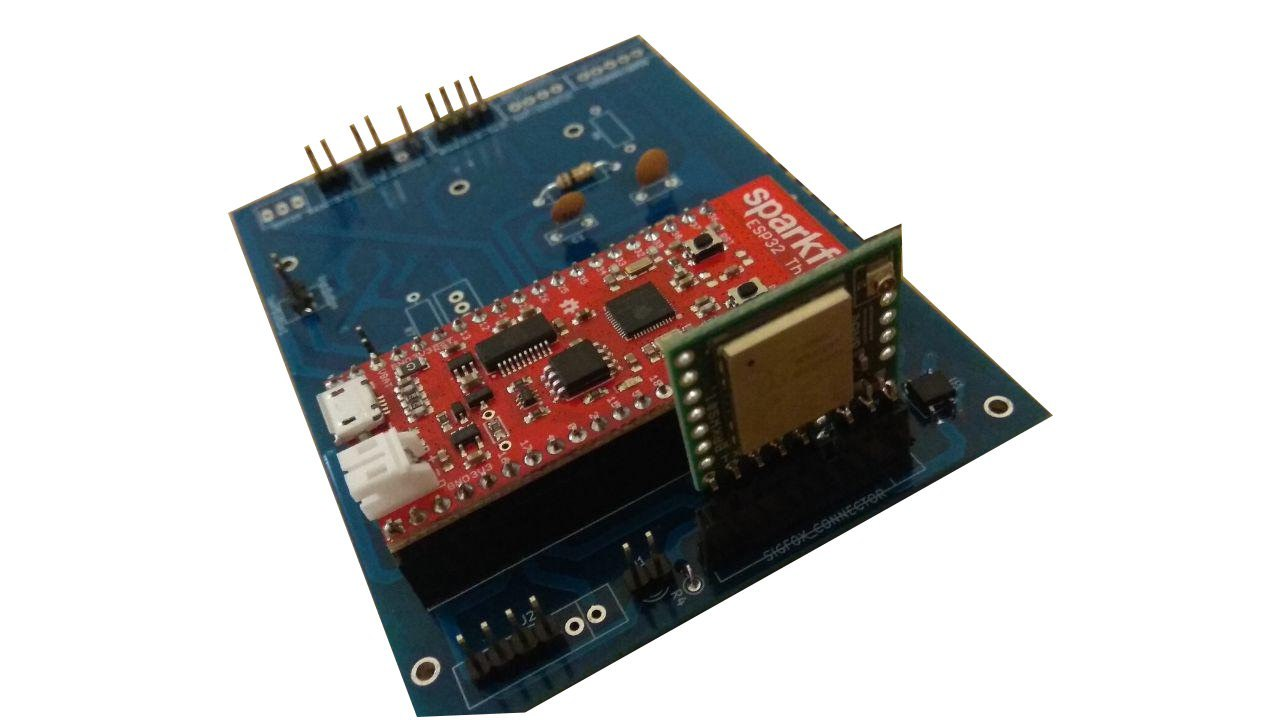
\includegraphics[scale=.15]{lcn_board.jpg} % angle=270,scale=0.35
    \caption{Electronics of the low-cost station.}
    \label{fig:station}
\end{figure}

\subsection{Station design}
The electronics of the station is shown in \cref{fig:station} The core of the measurement station is the Espressif ESP32 System-on-Chip \cite{espressif:sparkfun}. This board offers specific features for low-power IoT designs, such as a deep sleep stand-by mode. The board provides a dual-core 32-bit processor operating at the relatively low frequency of \SI{240}{\mega\hertz}, \SI{520}{\kilo\byte} of internal static RAM for storing the application code, and several peripherals which have been useful for the design of the agroclimatic station. One of such peripherals is the non-volatile flash memory, which contains the log of the measurements performed in a human-readable format. %Since each measurement currently takes \SI{37}{\byte}, and the flash memory is \SI{4}{MB} in size, the station can store more than two years of data.

% Furthermore, the board includes a Bluetooth module. This feature has been exploited to develop an Android application for on-site diagnosis of the station, calibration of the sensors and visualization of measured data. Measurement can also be downloaded via Bluetooth on the mobile device running the application.

The station is currently equipped with three sensors. A digital sensor provides the values of air temperature and air humidity. %, with an average accuracy of \SI{0.5}{\celsius} for the former and \SI{4,5}{\%} for the latter \cite{sensirion:sht10-temp-hum}. 
A Waspmote complex digital sensor is used to compute rainfall, wind direction, wind speed and wind gusts \cite{libellium:ws3000}. Lastly, a standard, analogic sensor is used to measure leaf wetness \cite{vaisala:yl83-leaf-wetness}. This sensor takes advantage of the ADC included in the ESP32 microcontroller.

% Electronics is packaged in a tailored, durable and 3D-printed case specifically designed to provide support for sensors and electronic equipment and to protect them from atmospheric weathering (\cref{fig:tailored-case}).
% \begin{figure}
%     \centering
%     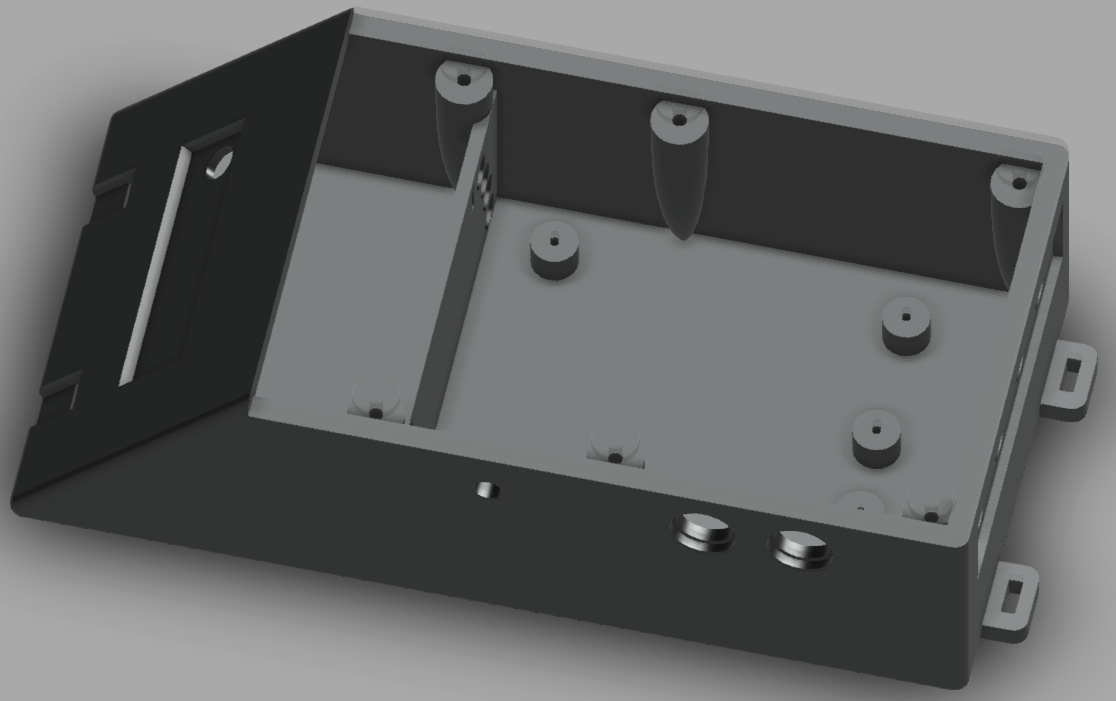
\includegraphics[scale=.20]{tailored-case.png} % angle=270,scale=0.35
%     \caption{Case specifically designed for the low-cost station.}
%     \label{fig:tailored-case}
% \end{figure}

The station is currently programmed to provide measurements on a 10-minute basis, and to stay active only during the data capturing phase, which takes less than 20 seconds. This means that the whole station is active for the \SI{3}{\%} of the time. For the remaining \SI{97}{\%} of the time, the station is in deep sleep mode, so as to save a huge share of energy. % In order to improve the accuracy of the wake-up cycle, an external \emph{Real-Time Clock} with an independent battery \cite{maxim:rtc} has been added to the design.

The data capturing phase includes also the time required for the transmission of the performed measurement to the database server. To this end, the station is equipped with a Sigfox network chip \cite{sigfox:module}. The stations are currently programmed to transmit the measurements synchronously, in order to allow real-time processing and publishing of data.

The station is powered by a \SI{3.7}{\volt}, \SI{3300}{\milli\amperehour} internal battery. Thanks to the aforementioned operation time optimisation, the battery has been proven to be able to provide about 25 days of lifetime without being charged. This budget is only used in dark hours, thanks to a solar panel which the station is equipped of. 
The complete recharge of the internal battery % by the solar panel
during daylight hours has been shown by on-field tests.

\subsection{Network infrastructure}
The proposed station can be effectively used to deploy a monitoring network, the architecture of which is shown in \cref{fig:network}. Apart from the stations, it includes a database server to store, process and publish data. 
It relies on the Sigfox cloud network \cite{sigfox:network-architecture} for communication between the stations and the network database.

\begin{figure}
    \centering
    \includegraphics[scale=.2]{Low-cost_network.png}
    \caption{Architecture of the proposed Low-Cost monitoring Network (LCN)}
    \label{fig:network}
\end{figure}
Data are sent by each station to the Sigfox backend server in the cloud, which is programmed to forward the station's data to the network database, by means of a callback. The network database is currently located on the premises of the Department of Agriculture of the University of Naples Federico II. 
Nevertheless, the database is developed inside a Docker container \cite{docker:mainpage}, so as to be easily relocated.

The use of the Sigfox network comes with some limitations, partly due to the subscription plan associated with the network chip.
To go into detail, only 140 messages per day are allowed from each network chip, and therefore from each station. 
This is not a particularly severe limitation, since measurements are performed on a 10-minute basis, stored on local non-volatile memory and then synchronously sent to the network database. 
The mentioned limitation means that, of the  \(6\times 24 = 144\) daily measurements, 4 are not sent but stored locally.

The limitation on the size of the message is more challenging. 
Each message is limited to \SI{96}{\bit} in size. 
It is worth mentioning that this limitation is imposed by the Sigfox network irrespectively of the subscription plan chosen \cite{sigfox:network-architecture}, although it could be overcome by sending more than one Sigfox message per measurement, were additional messages to be available. 
To cope with this extremely reduced message size, a compressed encoded representation of the measured data has been developed. 

\begin{figure}
    \centering
    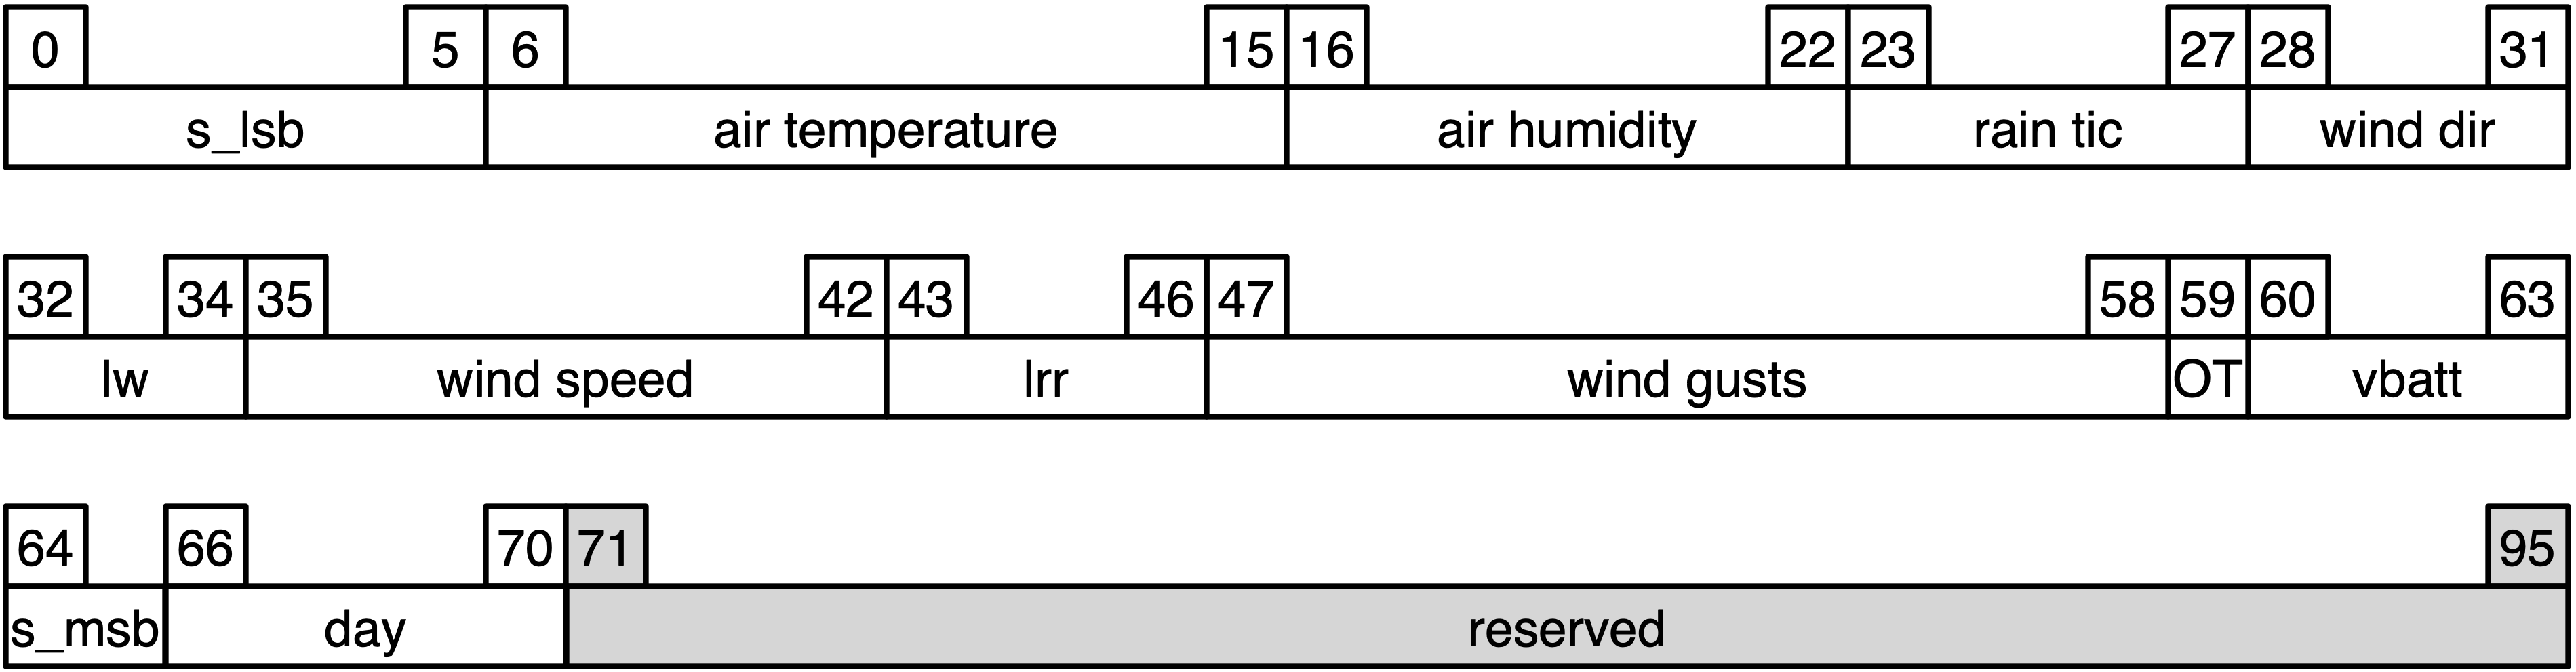
\includegraphics[scale=.55]{message_format.png}
    \caption{Format of the message sent by each station}
    \label{fig:message-format}
\end{figure}

The message format is shown in \cref{fig:message-format}. 
It is worth noting that the data compression is almost lossless for all but one climatic parameters. 
Namely, for wind gusts and wind direction, all the available information  is included in the message, whereas for air temperature, wind speed and rainfall a compression of the original data size is obtained by observing that the physical range of the climatic variables is actually smaller than the range of the sensors itself. 
For instance, range of the air temperature sensor goes from \SI{-40}{\celsius} to over \SI{120}{\celsius}, while the maximum air temperature on Earth does not exceed \SI{60}{\celsius} \cite{court:max-temp,roof:max-temp}. 
This means that a range of \SIrange{-40}{60}{\celsius} is sufficient not to lose any information. 
Such a range, at the resolution of \SI{0.1}{\celsius}, requires \SI{10}{\bit} to represent its 1000 distinct values. 
Only the leaf wetness has been subject to a quite severe compression. % since this information is commonly stored as Boolean (presence / absence) and then integrated over time (amount of uninterrupted time with wetness, expressed in minutes).
In fact, what is commonly measured  for the leaf wetness  is just the presence or absence of wetness at a given time, in order to compute later the amount of uninterrupted time with wetness.
The original measurement is rounded into seven equally spaced values between \SIrange{0}{100}{\%}.



% The network database is accessed by a custom PHP script, which upon reception of data from the Sigfox server, decodes the data string and insert both encoded and decoded data into the database. The storing of the encoded data string makes it possible to repeat the data parsing at a later moment, therefore only the encoded data string needs to be saved for backup purposes.

\section{Results}

\begin{figure}
    \centering
    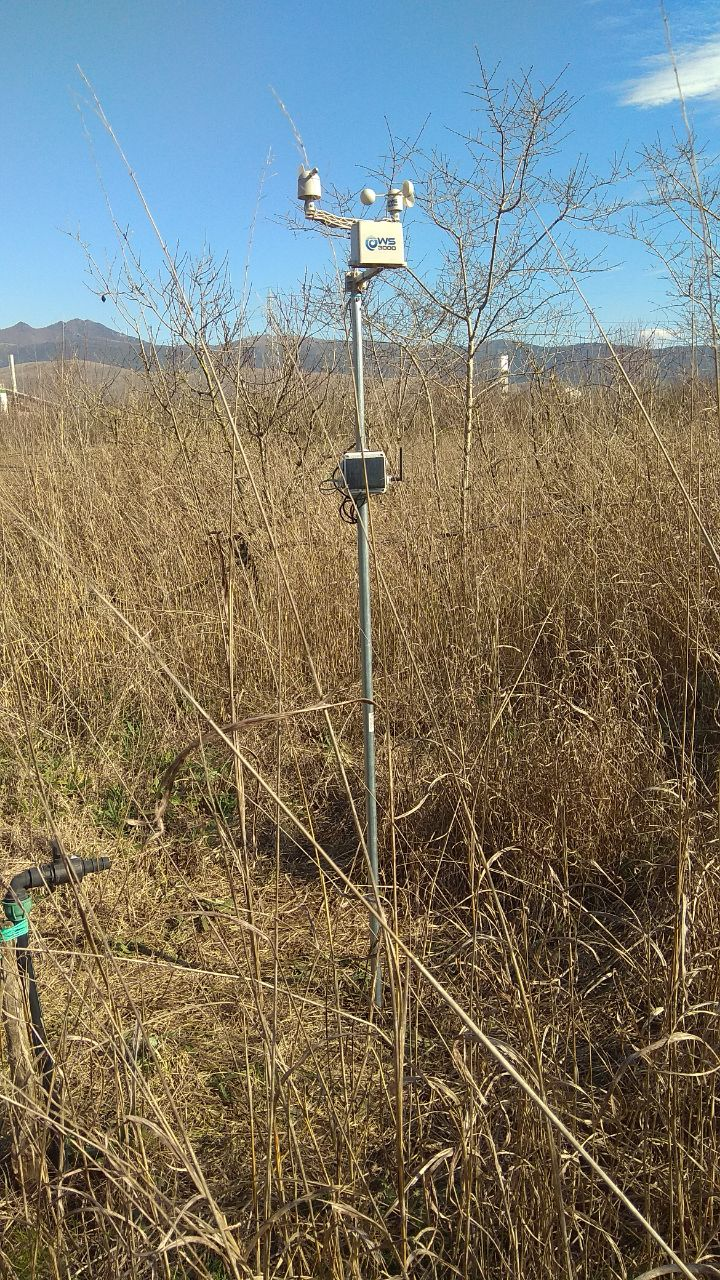
\includegraphics[scale=.25]{deployment_pignataro.jpg}
    \caption{Station installed for validation purposes}
    \label{fig:deployment}
\end{figure}


In order to validate the measurements provided by the proposed station, one prototype has been deployed in proximity of a permanent RAR station, located in the town of Pignataro Maggiore (CE), at N \ang{41;9;57.95} E \ang{14;8;59.08}.

The deployment of the prototype took place on February \nth{15}, 2019,  therefore the first complete month of data available is March. 
\cref{fig:10minutes} shows the monthly average of daily air temperature on 10-minute time scale for two full months, whereas \cref{fig:hourly} shows the monthly averages of daily mean air temperature, on an hourly time scale.

From \cref{fig:10minutes} it is clear that the proposed station follows closely the trend of air temperature, in fact, the graph of the proposed station exactly matches the shape of the reference station. Nevertheless, it is clear from \cref{fig:10minutes,fig:hourly} that there are issues to be addressed. 

The first problem is a calibration issue. The curves of the low-cost station are scaled compared to the reference curves, suggesting that the air temperature sensor is currently too much sensitive. This can be solved by properly tuning the calibration parameters of the low-cost station.

Another issue is linked to solar exposure.
From \cref{fig:10minutes,fig:hourly} it emerges that the error during the hours of maximum temperature is higher, of around \SI{1}{\celsius}, than the error during the hours of minimum temperature. 
This error is likely due to the fact that the air temperature sensor is incorrectly placed under direct solar radiation exposure, which means that the sensor overheats. 
This is going to be solved by using a proper encapsulation for the air temperature sensor.

It is worth noting that the discrepancy between data produced by the proposed station and the official data from the RAR station can be explained by deployment incorrectness. which can be fixed without altering the design of the station itself. This suggests that, after a calibration work which will be done later during the URCoFi aagroclimatic and pest monitoring work package, the proposed low-cost station will be able to provide reliable air temperature data.

\begin{figure}
    \centering
    \subfloat[March 2019]{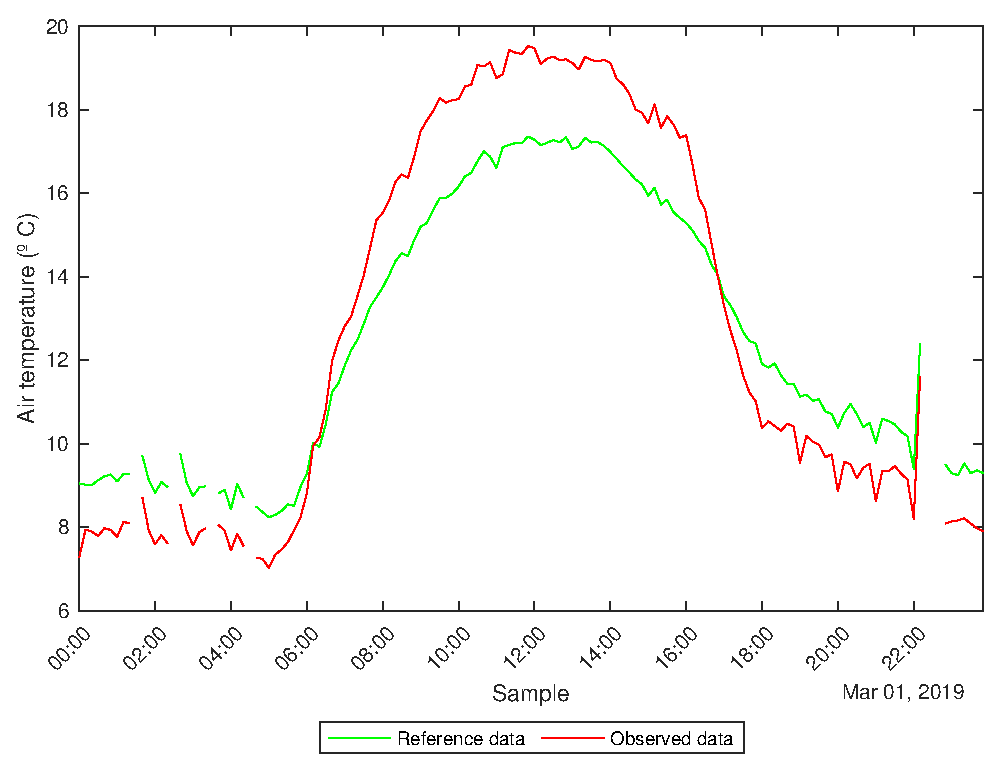
\includegraphics[height=0.11\paperheight]{March_10_minute_avg_air_temperature.eps}}
    \hspace{5mm}
    \subfloat[April 2019]{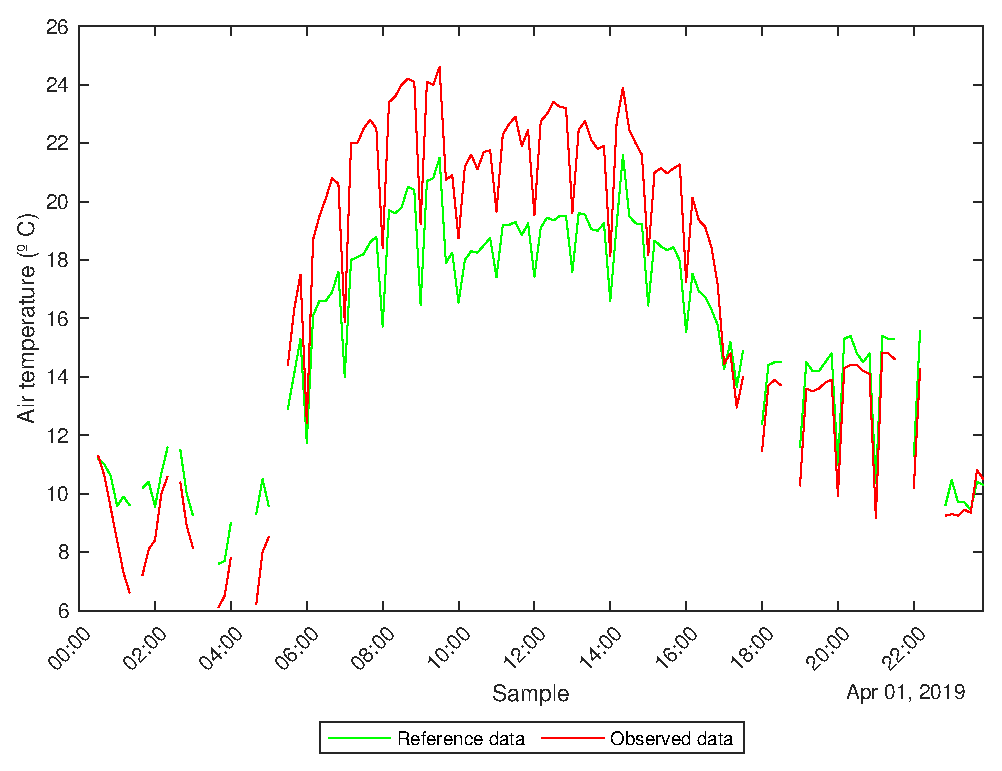
\includegraphics[height=0.11\paperheight]{April_10_minute_avg_air_temperature.eps}}
    \caption{Daily air temperature on 10-minute time scale, monthly averaged}
    \label{fig:10minutes}
\end{figure}
%
\begin{figure}
    \centering
    \subfloat[March 2019]{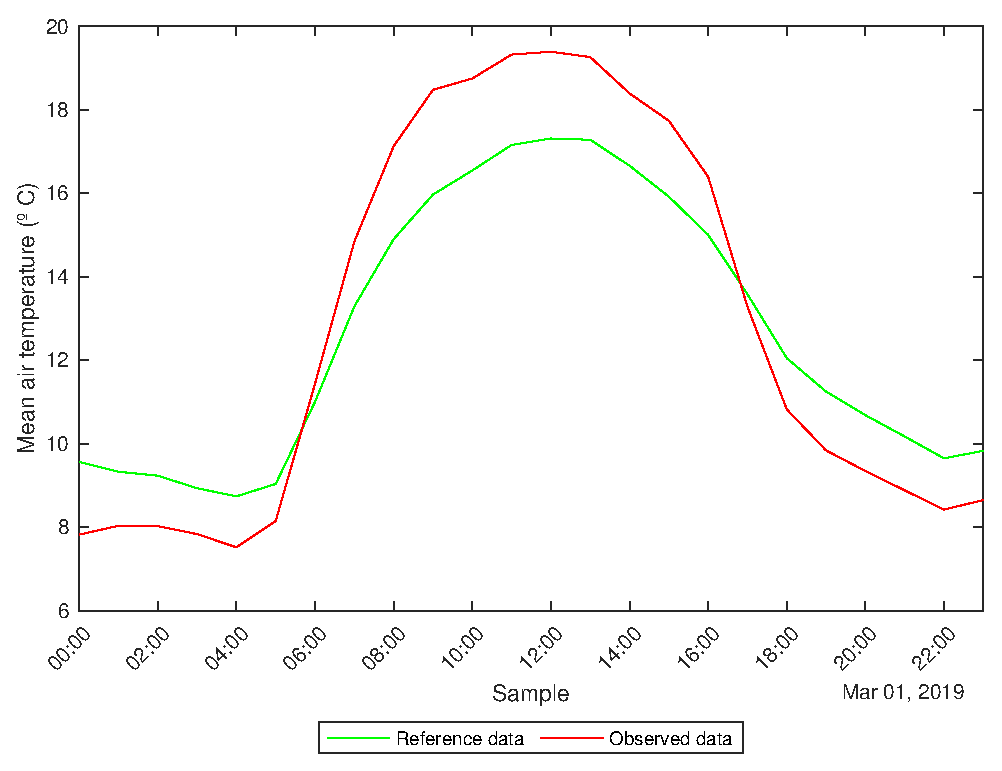
\includegraphics[height=0.1\paperheight]{March_hourly_avg_mean_air_temperature.eps}}
    \hspace{5mm}
    \subfloat[April 2019]{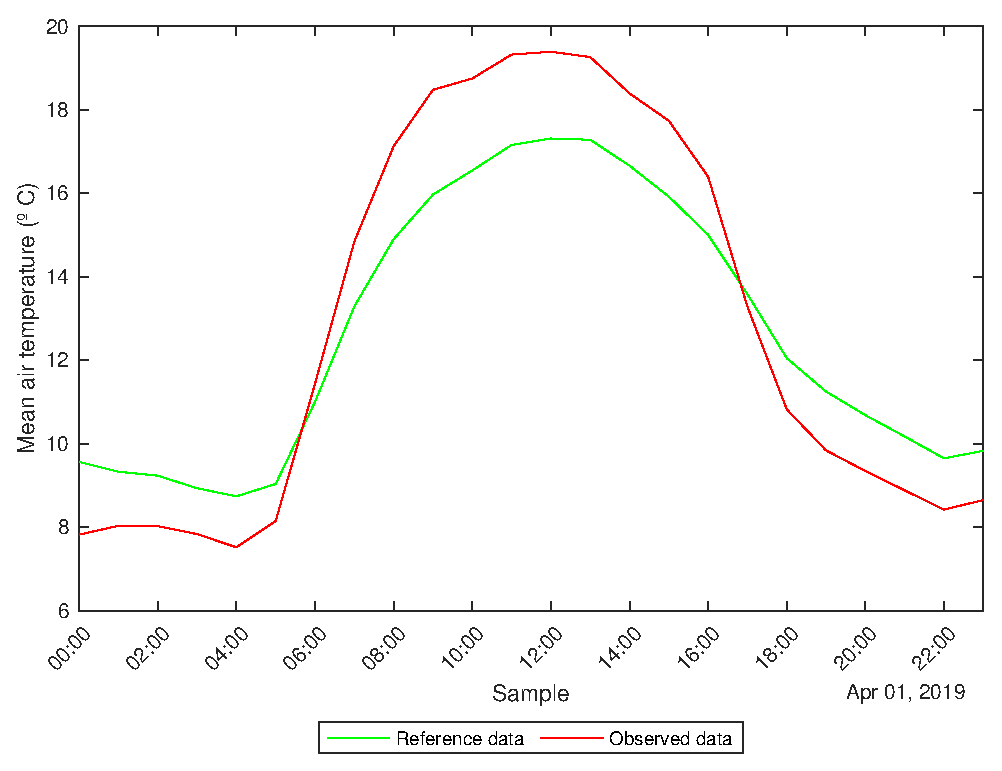
\includegraphics[height=0.1\paperheight]{April_hourly_avg_mean_air_temperature.eps}}
    \caption{Daily mean air temperature on hourly time scale, monthly averaged}
    \label{fig:hourly}
\end{figure}

\section{Conclusions}
The first evaluation of the proposed design for a low-cost, movable agroclimatic station is quite promising. Initial results indicate that the proposed station has the potential to closely reproduce the trend of air temperature as captured by the permanent stations, with sufficient  accuracy for the various usages of the agrometereological data.

Apart from the test prototype, two other stations have been deployed at the premises of private farm firms, confirming their interest in contributing to the agroclimatic network if presented with a small, movable and affordable station.

\subsection{Future Work}
The work proposed in this paper is only the initial step. The next step is the adjustment of the test prototype deployment in order to obtain more accurate air temperature data. Then, the analysis will be extended to the other measured variables in order to have a complete reliable station.

The following task under the agroclimatic and pest monitoring work package will involve the characterisation of pest risk models with data coming from the proposed low-cost station. To this end, a number of low-cost stations will be assembled and deployed in a localized area, and the data will be used to tune the parameter of pest risk models.

In addition, the low-cost station will be further developed to become capable of measuring all the fundamental climatic variables. 
This means that sensors for the remaining variables will be selected and assembled with the station, the firmware will be updated accordingly, and the data string format will be augmented to accomodate the new information.

Finally, data of the low-cost stations network will be integrated with data coming from the network of permanent stations, to provide a comprehensive view of the agroclimatic monitoring of the territory, and to allow subsequent operations over climatic data to operate seamlessly with both type of data. This further processing includes the execution of pest risk models, but also other applications like the building of digital climatic maps.

\section*{Acknowledgements}
This work has been funded by the Department of Agriculture of the Campania Region, within the URCoFi Executive Plan 2018-2019.

\printbibliography
\end{document}
